% Section content template for individual Educative lessons
% This file contains the actual content for a specific section
% Generated from Educative API section content

% Section: System Design: Uber
% Section ID: 6344806557286400
% Section Slug: system-design-uber
% Generated: 2025-12-07T23:30:16.636752

\subsection{What is Uber?}\label{fGq1eM2defSp5RHBUy7Cb}
\\
\textbf{Uber} is an application that provides ride-hailing services to its users. Anyone who needs a ride can register and book a vehicle to travel from source to destination. Anyone who has a vehicle can register as a driver and take riders to their destination. Drivers and riders can communicate through the Uber app on their smartphones.

\begin{figure}[htbp]
 \centering
 \begin{subfigure}[b]{0.48\textwidth}
 \centering
 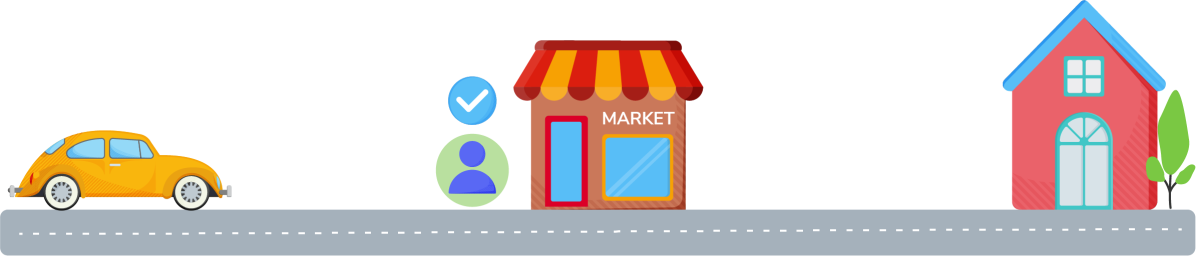
\includegraphics[width=\textwidth]{Images/chapter_30/section_6344806557286400/6048342698754048.png}
 \caption{A user requests a ride}
 \end{subfigure}
 \hfill
 \begin{subfigure}[b]{0.48\textwidth}
 \centering
 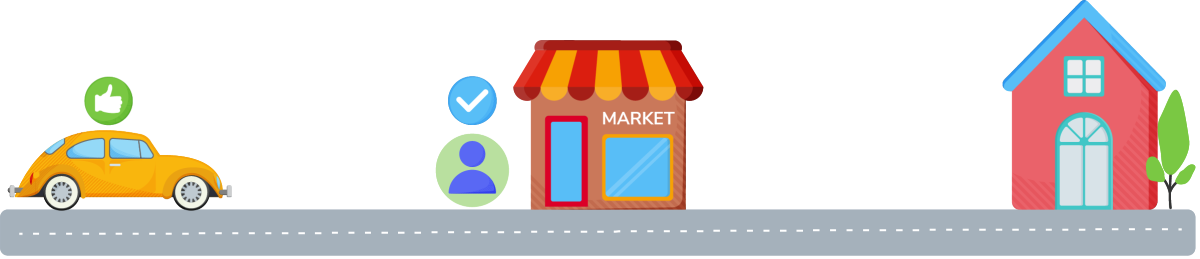
\includegraphics[width=\textwidth]{Images/chapter_30/section_6344806557286400/4517164292374528.png}
 \caption{Nearby drivers receive the request; one of them accepts it}
 \end{subfigure}
\end{figure}

\begin{figure}[htbp]
 \centering
 \begin{subfigure}[b]{0.48\textwidth}
 \centering
 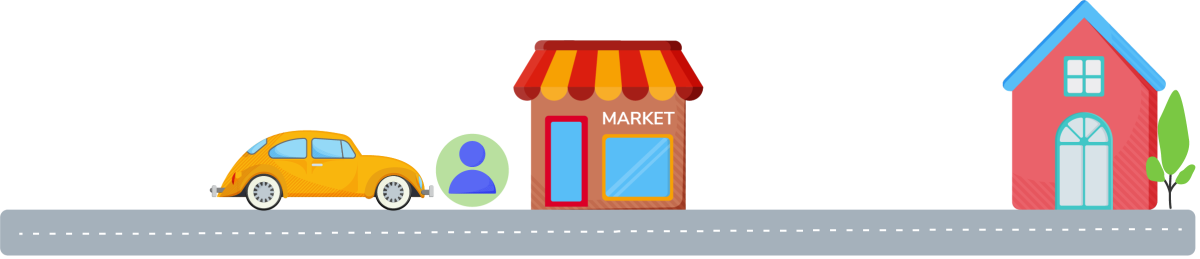
\includegraphics[width=\textwidth]{Images/chapter_30/section_6344806557286400/5198735135604736.png}
 \caption{The selected driver picks up the user from the specified location}
 \end{subfigure}
 \hfill
 \begin{subfigure}[b]{0.48\textwidth}
 \centering
 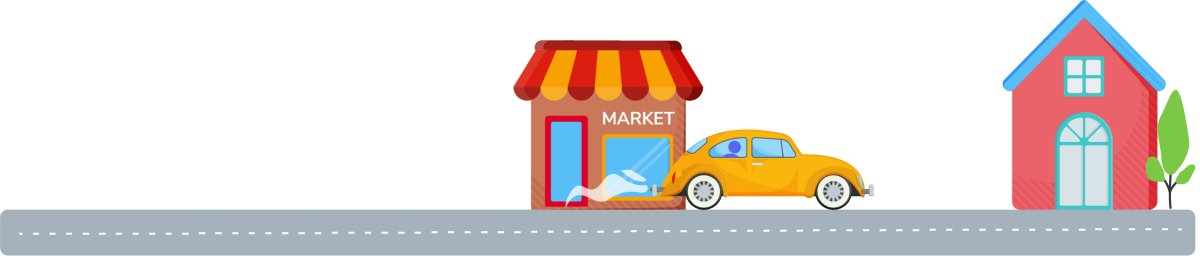
\includegraphics[width=\textwidth]{Images/chapter_30/section_6344806557286400/6342441842638848.png}
 \caption{The driver moves toward the desired destination}
 \end{subfigure}
\end{figure}

\begin{figure}[htbp]
 \centering
 \begin{subfigure}[b]{0.48\textwidth}
 \centering
 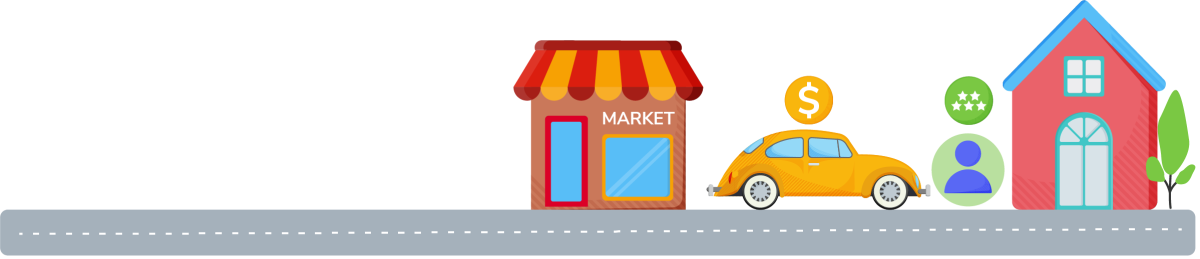
\includegraphics[width=\textwidth]{Images/chapter_30/section_6344806557286400/6407632668196864.png}
 \caption{The driver drops off the user, ends the ride, and receives payment}
 \end{subfigure}
\end{figure}

The illustration below shows the number of active users of Uber from the start of 2017 to 2020 (source: Statista):

\textit{\small [Chart data presented in table format]}

\begin{table}[htbp]
\centering
\small
\adjustbox{max width=\textwidth}{
\begin{tabular}{|p{0.475\textwidth}|p{0.475\textwidth}|}
\hline
\textbf{Label} & \textbf{Quaterly active users in millions} \\
\hline
\hline
Q1'17 & 49 \\
\hline
Q2'17 & 57 \\
\hline
Q3'17 & 62 \\
\hline
Q4'17 & 68 \\
\hline
Q1'18 & 70 \\
\hline
Q2'18 & 76 \\
\hline
Q3'18 & 82 \\
\hline
Q4'18 & 91 \\
\hline
Q1'19 & 93 \\
\hline
Q2'19 & 99 \\
\hline
Q3'19 & 103 \\
\hline
Q4'19 & 111 \\
\hline
Q1'20 & 103 \\
\hline
Q2'20 & 55 \\
\hline
Q3'20 & 78 \\
\hline
Q4'20 & 93 \\
\hline
\end{tabular}
}
\caption{Monthly number of Uber's active users worldwide from 2017 to 2020(by quarter)}
\end{table}

Let's evaluate your understanding of the functional and nonfunctional requirements for Uber. Identify \textbf{three functional and three nonfunctional requirements} for Uber in the widget below. Provide the need for each requirement in a single line.

\textbf{Question:}

Identify the functional and nonfunctional requirements for Uber.

\textbf{Reference Answer:}

The functional requirements are: 1- Update driver location: The driver is a moving entity, so the driver's location should be automatically updated at regular intervals. 2- Find nearby drivers: The system should find and show the nearby available drivers to the rider. 3- Request a ride: A rider should be able to request a ride, after which the nearest driver should be notified about the rider's requests. 4- Manage payments: At the start of the trip, the system must initiate the payment process and manage the payments. 5- Show driver estimated time of arrival (ETA): The rider should be able to see the estimated time of arrival of the driver. 6- Confirm pickup: Drivers should be able to confirm that they have picked up the rider. 7- Show trip updates: Once a driver and a rider accept a ride, they should be able to constantly see trip updates like ETA and current location until the trip finishes. 8- End the trip: The driver marks the journey complete upon reaching the destination, and they then become available for the next ride.

\subsection{How will we design Uber?}\label{EjlONe_YF4hyWafN5MQ5k}
\\
There are many unanswered questions regarding Uber. How does it work? How do drivers connect with riders? These are only two of many. This chapter will design a system like Uber and find the answer to such questions.
\\
We've divided the design of Uber into six sections:

\begin{enumerate}
\item
\protect\phantomsection\label{mK6g3EvpBa5OsUNBgtlP7}
\href{https://www.educative.io/courses/grokking-the-system-design-interview/requirements-of-ubers-design}{\textbf{Requirements}}\textbf{:} This lesson will describe the functional and non-functional requirements of a system like Uber. We'll also estimate the requirements of multiple aspects of Uber, such as storage, bandwidth, and the computation resources.
\item
\protect\phantomsection\label{R26znwKKzSq3iYugC3k_c}
\href{https://www.educative.io/courses/grokking-the-system-design-interview/high-level-design-of-uber}{\textbf{High-level Design}}\textbf{:} We'll discuss the high-level design of Uber in this lesson. In addition, we'll also briefly explain the API design of the Uber service.
\item
\protect\phantomsection\label{SZqjAvc6PBoVyokfkOnmZ}
\href{https://www.educative.io/courses/grokking-the-system-design-interview/detailed-design-of-uber}{\textbf{Detailed Design}}\textbf{:} We'll explore the detailed design of Uber in this lesson. Moreover, we will also discuss the working of different components used in designing Uber.
\item
\protect\phantomsection\label{98Vv5bub0ZiZOccivrnWY}
\href{https://www.educative.io/courses/grokking-the-system-design-interview/payment-service-and-fraud-detection-in-uber-design}{\textbf{Payment Service and Fraud Detection}}\textbf{:} We'll learn how the payment system works in Uber design. Moreover, we'll also discuss how we can catch different frauds related to payments in Uber-like systems.
\item
\protect\phantomsection\label{ouziJsOt3AEnZAfxGzNwl}
\href{https://www.educative.io/courses/grokking-the-system-design-interview/evaluation-of-ubers-design}{\textbf{Evaluation}}\textbf{:} This lesson will explain how Uber can fulfill all the non-functional requirements through the proposed design.
\item
\protect\phantomsection\label{3idZ0obbO2V-t-_9TdSXz}
\href{https://www.educative.io/courses/grokking-the-system-design-interview/quiz-on-ubers-design}{\textbf{Quiz}}\textbf{:} We'll reinforce major concepts of Uber design via a quiz.
\end{enumerate}
\\
Let's go over the requirements for designing a system like Uber in the next lesson.

% End of section content